With various methods of ML being applied to all manner of things to try and help make predictions about life better, it is only natural that the data in question will include personal data. Whether this is through monitoring app/website usage or very simply tracking what people ``like" or send to each other, the data is personal to each user and as such the experience of each user is personal. \\ \\
However, data can stray beyond this into more truly personal information such as that of the medical nature.
This is trickier to deal with, given that medical data is very tightly controlled and restricted due to its highly sensitive nature and the governing bodies controlling it are usually very unwilling to share. 
Now in the past this wasn't really an issue as typically only medical professionals of the governing organisation (e.g. the National Health Service (NHS)) would want access to this data and actually have any good reason. 
So it was very easy and efficient to deny any external access. 
However, we now live in a world where the prevalence of ML has made external researchers' access to data increasingly valuable to society. 
Users, beyond medical professionals, want access to this highly sensitive data to try and make the world a better place.
\\ \\
Whether this is in trying to train a model to recognise cancerous cells or early onset dementia, data surrounding that is needed to accurately make these predictions. 
So, to be able to push the field of medicine forward and to leverage to full power of modern day computing, we as software engineers need access to this data. 
So several methods of trying to preserve the privacy of the users of this data have been created to tackle this.

\subsection{Homomorphic Encryption}
Encrypting data seems to be a fairly intuitive starting point for trying to keep the privacy of user's data secured. 
For cloud computing \cite{cloud_fhe}, it is almost a necessity that the data is encrypted in some manner as otherwise employees of the company potentially have access to this data and could act maliciously \cite{access_private}. 
However, it results in a system where no one can read or understand the data without the appropriate decryption keys (usually not stored on a centralised server) and so trying to perform any calculations or processing on the data is somewhat redundant. 
So in comes the idea of Homomorphic Encryption. This is a style of encrypting data such that you are able to perform some given calculation on the encrypted data without the need for decrypting it first (e.g. addition).
\\ \\ 
However, only being able to perform 1 operation on the data isn't particularly useful and so the more impressive standard of Fully Homomorphic Encryption (FHE) was postulated \cite{fhe}. 
In theory, FHE allows for any number of operations to be performed (although current operations are typically just addition and multiplication) on the encrypted data. 
However, it is not a simple/intuitive system to implement for any given task and so for certain tasks, it may not be an ideal method on preserving the privacy of data.


\subsection{K-Anonymisation}
The idea behind anonymising data is to not be able to associate an individual person's data record with their actual identity in a given dataset. 
This helps to reassure that the data will not cause any worry or harm to that individual. This has the added side-effect of no longer making the data personal anymore and so more freely able to be used beyond the governing owner of that data. 
This is hugely beneficial to both parties and is a great starting point for preserving the privacy of the data. 
\\ \\
However, this is not as simple as it sounds and many attempts to pseudo-anonymise the data have resulted in people able to use more than one available dataset to link medical data with more available (and less sensitive) data like a voter list \cite{failed_anonymisation}.
\\ \\
Even if that weren't the case, you get certain attributes that when taken together are potentially able to identify a person. These are called quasi-identifiers. 
An example would be if you knew their post code and their date-of-birth, you could potentially figure out a disease they have if no one in that postcode shares that date-of-birth with them. e.g. id=3 in Table \ref{tbl:pre-anon}.
\\ \\
A way to tackle these is through the use of k-anonymising the data. A table of data is k-anonymous if every record in the table is indistinguishable from at least k-1 other records, with respect to every set of quasi-identifiers (not something that is itself a unique identifier, but when paired with other quasi-identifiers it can identify someone). 
The 2 styles of doing this are perturbative methods and non-perturbative methods but seeing as perturbative methods (e.g. adding noise) does not retain data integrity, we won't be considering it. 
Two main ways of achieving k-anonymity for non-perturbative methods are generalising the data (replacing attribute values with something more generalised e.g. 54321 $\longrightarrow$ 54***) and suppression (deletion of row or column e.g. row with id=3 in Table \ref{tbl:pre-anon}).
\begin{center}
    \begin{longtable}{ |c|c|c|c|c| }
    \caption{Pre-Anonymisation}
    \label{tbl:pre-anon}
    \hline
    \textbf{id} & \textbf{sex} & \textbf{DoB} & \textbf{postcode} & \textbf{disease} \ \\ \hline
    1 & female & 1998-03-13 & SW7 2BU & anxiety \ \\ \hline
    2 & female & 1998-10-27 & NW1 9LJ & anxiety \ \\ \hline
    3 & female & 1997-01-22 & AL9 7TA & chicken pox \ \\ \hline
    4 & male & 1999-11-11 & HP11 1UA & ADD \ \\ \hline
    5 & male & 1999-06-18 & HP14 4JQ & Dyspraxia \ \\ \hline
    6 & male & 1999-06-21 & HP11 2DQ & ADHD \ \\ \hline
    \end{longtable}
    
    \begin{longtable}{ |c|c|c|c|c| }
    \caption{2-Anonymised}
    \label{tbl:2-anon}
    \hline
    \textbf{id} & \textbf{sex} & \textbf{DoB} & \textbf{postcode} & \textbf{disease} \ \\ \hline
    \rowcolor{lightgray} 1 & female & 1998 & London & anxiety \ \\ \hline
    \rowcolor{lightgray} 2 & female & 1998 & London & anxiety \ \\ \hline
    \rowcolor{gray} 4 & male & 1999 & High Wycombe & ADD \ \\ \hline
    \rowcolor{gray} 5 & male & 1999 & High Wycombe & Dyspraxia \ \\ \hline
    \rowcolor{gray} 6 & male & 1999 & High Wycombe & ADHD \ \\ \hline
    \end{longtable}
\end{center}

The data is still susceptible to homogeneity and semantic attacks [Table \ref{tbl:2-anon}] and while {l-Diversity} can fix the former there is never any guarantee that a dataset is 100\% completely and truly anonymised. With k-anonymisation, a specific data record can't be identified with any given individual but information can still be inferred. The governing body behind the data sometimes has to make a decision about what is an acceptable level of anonymisation without completely destroying any utility or functionality behind it. There are some techniques being investigated through clustering of the data to help minimise information loss \cite{anon_cluster} but again, these only go so far. It should also be noted that k-anonymity can only work on table and record style data instead of things like images and so has its limitations there.


\subsection{Secure Multi-Party Computation}
A different approach for preserving privacy is when you have multiple parties all wanting to calculate something based on each others' data but no one wants to share their data. For this we have Secure Multi-Party Computation (MPC) and it is when 2 or more parties share their data with a 3rd trusted party and it carries out an algorithm that doesn't reveal anything about the parties' data that was given (unless the result of the function revealed the values anyway). \\ \\
However this involves a trusted 3rd party and so a different style would be through something called Secret Sharing (SS) and will be explained through the BGW Protocol \cite{bgw}. This expresses the function that is computed as an arithmetic circuit containing addition and multiplication gates. It involves the parties splitting up their value into ``shares" and sending them off to the other parties. Each party then calculates the function on those shares, broadcasts the output as new shares before combining the shares it receives into a value. This is shown in Figure \ref{fig:bgw}.
\begin{figure}[htbp]
	\centering
    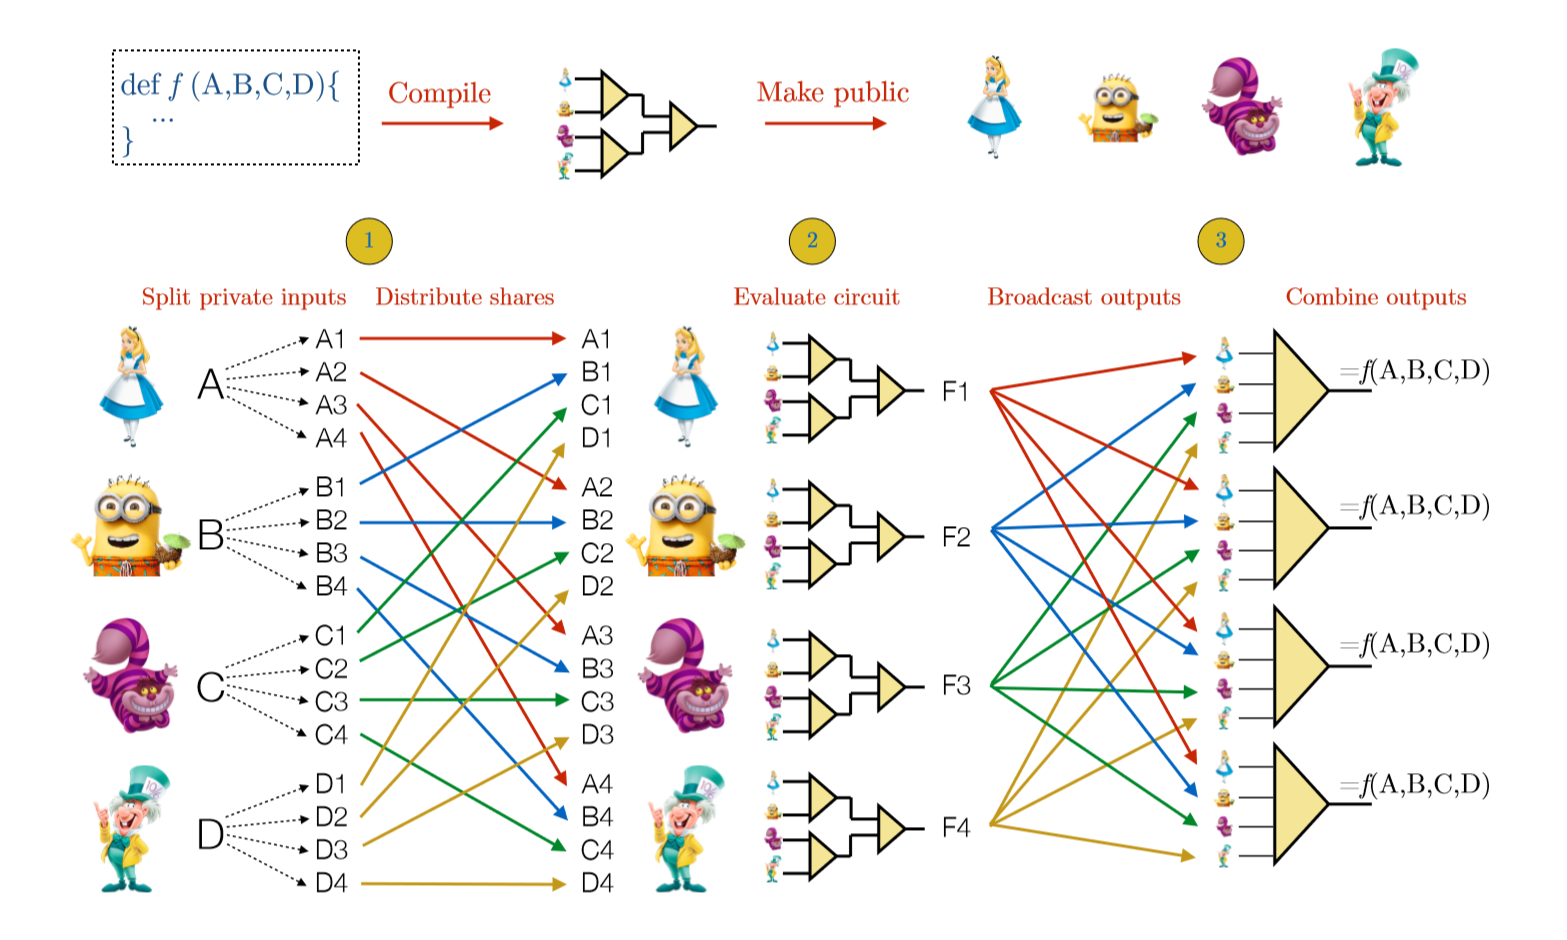
\includegraphics[scale=0.3]{background/bgw.png}
	\caption{BGW Protocol, courtesy of N. Dulay's Privacy Engineering Slides \cite{priv_eng}}
	\label{fig:bgw}
\end{figure}


\subsection{Differential Privacy}
Another method for preserving privacy is Differential Privacy (DP). DP guarantees that when you query a dataset D, the result that you get will be approximately the same (if not the same) irrespective of the presence of whether or not the dataset contained a certain value. This can be summarised as:
\begin{equation}
    Pr[x | y \in D] \approx Pr[x | y \notin D]
\end{equation}
As we want = instead of $\approx$ without destroying utility, we have the difference shown with $\epsilon$ such that:
\begin{equation}
    Pr[M(D) = y] \leq e^\epsilon Pr[M(D') = y]
\end{equation}
Where D is the dataset with no changes and D' is the dataset with the missing row. M is the function applied to D that computes the output and ensures privacy. We have to make sure that the two datasets satisfy the condition that they are neighbouring, i.e. they differ by exactly one row. This is what it means for a mechanism to be $\epsilon$-Differentially private. \\ \\
For achieving DP, the key ingredient is adding noise to the data until the above requirement is satisfied. This can be done with either Gaussian or Laplacian noise, with Laplace noise being the more common choice for DP. Typically, you draw from a Laplacian distribution that is $L(1/\epsilon)$ for the mechanism to remain $\epsilon$-Differentially private. Laplace's probability density function (pdf) is defined as:
\begin{equation}
    L(x|\mu,b) = \dfrac{1}{2b} \exp \left( -\dfrac{|x - \mu|}{b}\right)
\end{equation}

For ML models, depending on where we add the noise to, our mechanism will either be Locally or Globally differentially private. If the noise is added to the inputs of the model then it is Local DP. This involves each client adding noise so as to help protect their data. This helps ensure that each user has plausible deniability as you could never accurately claim that a certain client's specific data is of some specific value. If the noise is added to the end then it is Global DP. This is more desirable if the owner of the person taking the data and training with it is trustworthy as you can normally achieve more accurate results \cite{global_dp} as the input data has not been modified or changed. \\ \\
Interestingly, there are cases where adding noise to the gradient of models in very deep NNs \cite{dnn_noise} or as a form of regularisation for data augmentation \cite{robust_corrupt_noise} can help improve the generalisation performance of the trained model through either greater feature extraction ability or from reducing over-fitting.